\documentclass[10pt, landscape]{article}
\usepackage[scaled=0.92]{helvet}
\usepackage{calc}
\usepackage{multicol}
\usepackage{ifthen}
\usepackage[a4paper,margin=3mm,portrait]{geometry}
\usepackage{amsmath,amsthm,amsfonts,amssymb}
\usepackage{color,graphicx,overpic}
\usepackage{hyperref}
\usepackage{newtxtext} 
\usepackage{enumitem}
\usepackage[table]{xcolor}
\usepackage{mathtools}

\usepackage[outputdir=../]{minted} % for code syntax highlighting
\usepackage{mdframed} % framing, backgrounds

\setlist{nosep}

% for including images
\graphicspath{ {../images/}, {./images/} }

% \pdfinfo{
%   /Title (CS2100_midterms.pdf)
%   /Creator (TeX)
%   /Producer (pdfTeX 1.40.0)
%   /Author (Zeepheru)
%   /Subject ()
%   /Keywords ()}

% Turn off header and footer
\pagestyle{empty}

\newenvironment{tightcenter}{%
  \setlength\topsep{0pt}
  \setlength\parskip{0pt}
  \begin{center}
}{%
  \end{center}
}

% redefine section commands to use less space
\makeatletter
\renewcommand{\section}{\@startsection{section}{1}{0mm}%
                                {-1ex plus -.5ex minus -.2ex}%
                                {0.5ex plus .2ex}%x
                                {\normalfont\large\bfseries}}
\renewcommand{\subsection}{\@startsection{subsection}{2}{0mm}%
                                {-1explus -.5ex minus -.2ex}%
                                {0.5ex plus .2ex}%
                                {\normalfont\normalsize\bfseries}}
\renewcommand{\subsubsection}{\@startsection{subsubsection}{3}{0mm}%
                                {-1ex plus -.5ex minus -.2ex}%
                                {1ex plus .2ex}%
                                {\normalfont\small\bfseries}}%
\renewcommand{\familydefault}{\sfdefault}
\renewcommand\rmdefault{\sfdefault}
%  makes nested numbering (e.g. 1.1.1, 1.1.2, etc)
\renewcommand{\labelenumii}{\theenumii}
\renewcommand{\theenumii}{\theenumi.\arabic{enumii}.}
\renewcommand\labelitemii{•}
\renewcommand\labelitemiii{•}
%  convenient absolute value symbol
\newcommand{\abs}[1]{\vert #1 \vert}
%  convenient floor and ceiling
\newcommand{\floor}[1]{\lfloor #1 \rfloor}
\newcommand{\ceil}[1]{\lceil #1 \rceil}
%  convenient modulo
\newcommand{\Mod}[1]{\ \mathrm{mod}\ #1}
%  for logical not operator, iff symbol, convenient "if/then"
\renewcommand{\lnot}{\mathord{\sim}}
\let\then\rightarrow
\let\Then\Rightarrow
%  vectors
\newcommand{\vv}[1]{\boldsymbol{#1}}
\newcommand{\VV}[1]{\overrightarrow{#1}}
%  column vector
\newcommand{\cvv}[1]{\left(\begin{smallmatrix}#1\end{smallmatrix}\right)}
\newcommand{\code}[1]{\textcolor{myblue}{\texttt{#1}}}
\newcommand{\asm}[1]{\mintinline{asm}|#1|}
\newcommand{\java}[1]{\mintinline{java}|#1|}
\newcommand{\inline}{\mintinline[fontsize=\normalsize]{text}}
\newcommand\bggreen{\cellcolor{green!10}}

\makeatother
\definecolor{myblue}{cmyk}{1,.72,0,.38}
\everymath\expandafter{\the\everymath \color{myblue}}
% Define BibTeX command
\def\BibTeX{{\rm B\kern-.05em{\sc i\kern-.025em b}\kern-.08em
    T\kern-.1667em\lower.7ex\hbox{E}\kern-.125emX}}

% Don't print section numbers
\setcounter{secnumdepth}{0}

\setlength{\parindent}{0pt}
\setlength{\parskip}{0pt plus 0.5ex}
%% this changes all items (enumerate and itemize)
\setlength{\leftmargini}{0.5cm}
\setlength{\leftmarginii}{0.4cm}
\setlength{\leftmarginiii}{0.5cm}
\setlist[itemize,1]{leftmargin=2mm,labelindent=1mm,labelsep=1mm}
\setlist[itemize,2]{leftmargin=3mm,labelindent=1mm,labelsep=1mm}
\setlist[itemize,3]{leftmargin=3mm,labelindent=1mm,labelsep=1mm}

%My Environments
\newtheorem{example}[section]{Example}

% -----------------------------------------------------------------------

\begin{document}
\raggedright
\footnotesize
\begin{multicols}{2}

% multicol parameters
% These lengths are set only within the two main columns
\setlength{\columnseprule}{0.25pt} % column separator line
\setlength{\premulticols}{1pt}
\setlength{\postmulticols}{1pt}
\setlength{\multicolsep}{1pt}
\setlength{\columnsep}{2pt}

\begin{center}
    \fbox{%
        \parbox{0.8\linewidth}{\centering \textcolor{black}{
            {\Large\textbf{CS2100}}
            \\ \normalsize{AY24/25S1 Midterms}}
            \\ {\footnotesize By: \textcolor{myblue}{github.com/zeepheru}}
        }%
    }
\end{center}

% START CONTENT _________________________________>
\begin{center}
    \fbox{%
        \parbox{0.9\linewidth}{\centering \textcolor{black}{
            {\Large\textbf{EXAM INFO}}
            \\ $25$ 1-mark MCQ + $3$ 5-mark SRQ - 
            $~2$ mins \textbf{per mark!}
            \\ \textbf{SEAT:} MPSH2A, 68
            }
        }%
    }
\end{center}

\section{Number Systems}

\subsection{HEX QRF}

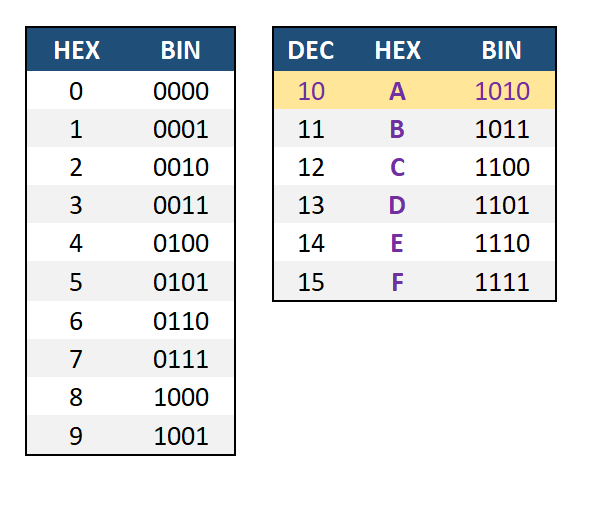
\includegraphics[width=0.8\linewidth]{cs2100/images/num-hex_bin.png}

\subsection{4-bit Signed Int}

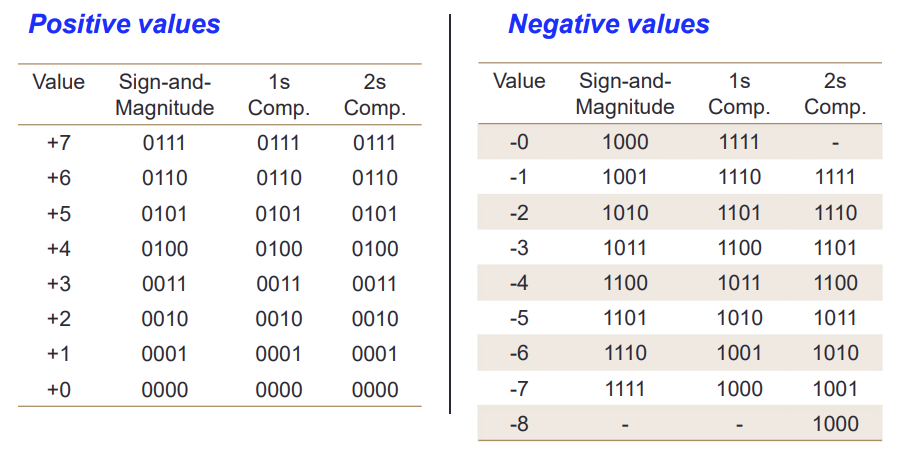
\includegraphics[width=1\linewidth]{cs2100/images/num-dec-4bit.png}

\subsection{Conversion}
\textbf{Base-R} to \textbf{decimal}: multiply digits with their corresponding weights. \\
\textbf{Decimal} to \textbf{base-R}
\begin{itemize}
    \item Whole numbers: repeated \textbf{division}-by-2
    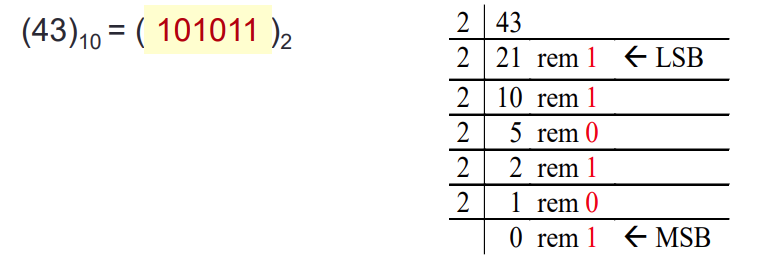
\includegraphics[width=0.8\linewidth]{cs2100/images/num-conv_wholenum.png}
    \item Fractions: repeated \textbf{multiplication}-by-2
    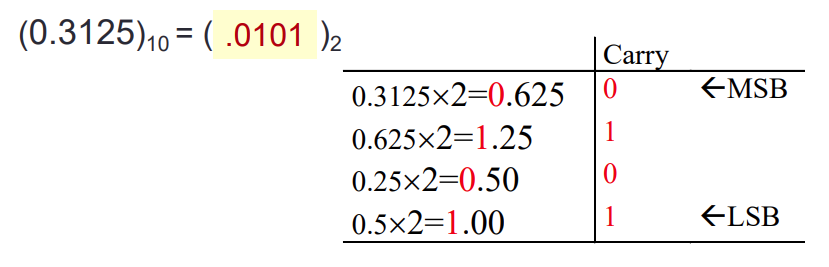
\includegraphics[width=0.8\linewidth]{cs2100/images/num-conv_frac.png}
\end{itemize}

\rule{\linewidth}{1pt}

\section{C}

\subsection{Arrays}
\begin{minted}{c}
#include <stdio.h>

void printArray(int *arr, int size) {
    int *ptr;  // Pointer to go through the array
    for (ptr = arr; ptr < arr + size; ptr++) {
        printf("%d\n", *ptr);
    }
}

int main() {
    int numbers[] = {10, 20, 30, 40, 50};
    int size = sizeof(numbers) / sizeof(numbers[0]);  
    printArray(numbers, size); 

    return 0;
}
\end{minted}

\section{MIPS - C Conversion}
\subsection{Conditionals}

\begin{itemize}
    \item \java{if (t0 < t1)}
    \begin{minted}{nasm}
    slt   $t2, $t0, $t1       
    bne   $t2, $zero, true_label 
    \end{minted}
    \item \java{if (t0 > t1)}
    \begin{minted}{nasm}
    slt   $t2, $t1, $t0       
    bne   $t2, $zero, true_label
    \end{minted}
    \item \java{if (t0 <= t1)}
    \begin{minted}{nasm}
    slt   $t2, $t1, $t0       
    beq   $t2, $zero, true_label
    \end{minted}
    \item \java{if (t0 >C= t1)}
    \begin{minted}{nasm}
    slt   $t2, $t0, $t1     
    beq   $t2, $zero, true_label
    \end{minted}
    
\end{itemize}

\rule{\linewidth}{1pt}

\section{ISA}

J-format instructions - 26-bit input, 28-bit total effective addressable range, 
take the first 4 bits of the calling address.

\section{MIPS}

\subsection{Syscalls}
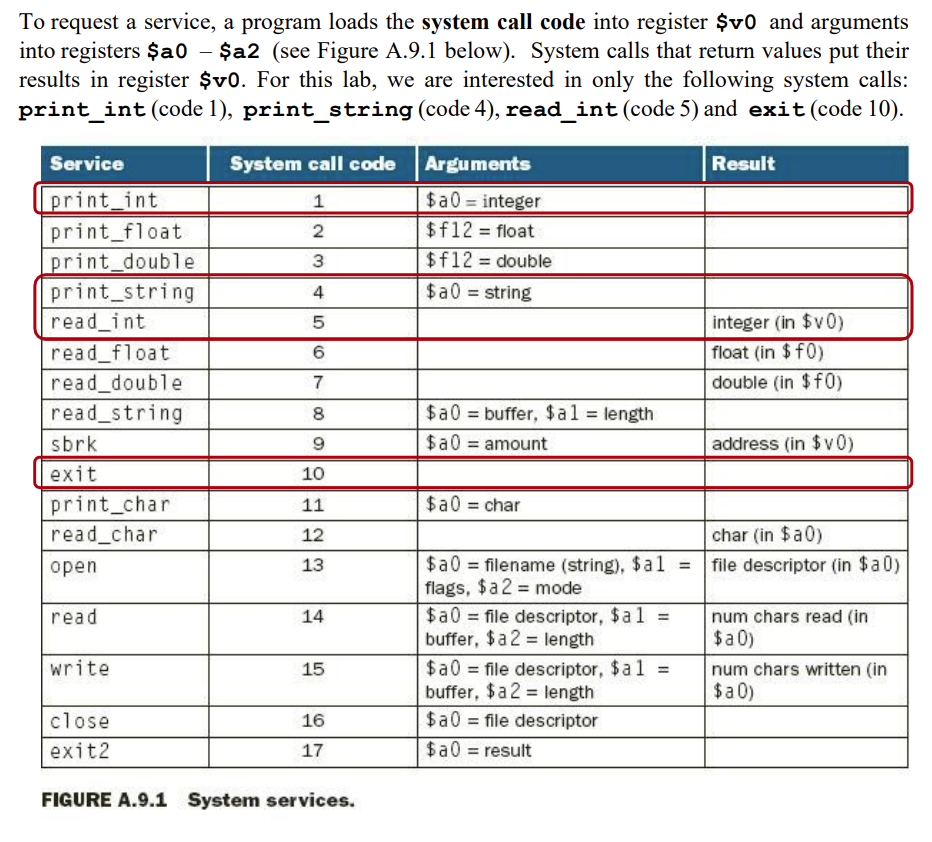
\includegraphics[width=\linewidth]{cs2100/images/mips-syscalls.png}
\begin{minted}{nasm}
li    $v0, 1    # syscall for print_int
li    $a0, 5    # int to print
syscall         # print
\end{minted}

\end{multicols}

\end{document}